\subsection{Listener-System}

\subsubsection{Aufgaben}
Da die verschiedenen Adapter Informationen über den aktuellen Zustand des Roboters von außen (Anwendung, Steuerung,...) erhalten, wird eine Möglichkeit benötigt mit der man den Adaptern den Abschluss von Befehlen mitteilen kann.

\subsubsection{Aufbau}
Die Idee dazu ist die Verwendung sogenannter Listener (von “to listen”, horchen) welche die Änderung des Zustands von außen ermöglichen. Jeder Adapter besitzt abhängig von seinem Typ einen entsprechenden Listener. Der Grund dafür ist das die Art der Kommunikation je nach Adapter unterschiedlich ist. So kommuniziert der VirtualAdapter lediglich über Events mit der Gegenseite, während der Edubot- und KEBA-Adapter über Netzwerk mit einer Steuerung kommunizieren. Um auch hier eine Erweiterung zu ermöglichen wird die abstrakte IStateListener definiert und von den Klassen VirtualStateListener und NetworkStateListener implement.

\begin{figure}[H]
  \centering
  \begin{minipage}[t]{12 cm}
  	\centering
  	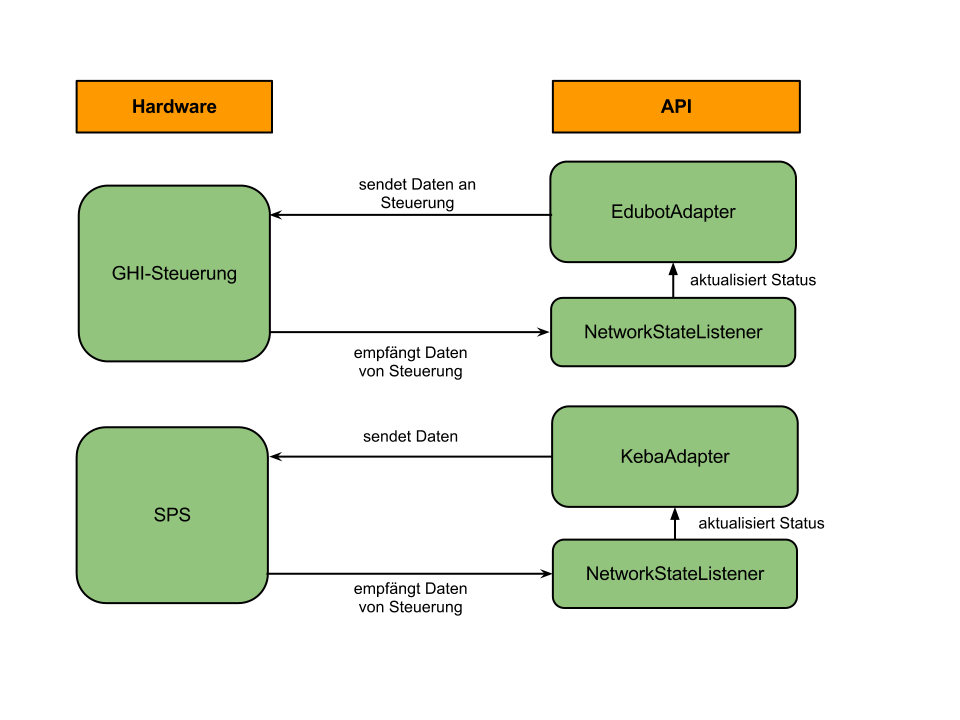
\includegraphics[width=12cm]{images/ListenerSystem} 
    \caption{Listener Konzept}
  \end{minipage}
\end{figure}

\subsubsection{Umsetzung}
\textbf{IStateListener}
\newline
Die abstrakte Klasse \textit{IStateListener} definiert die zu implementierenden Methoden in Hinsicht auf eine erfolgreiche Verwendung als Listener. Weiters benötigt ein Listener den Adapter dem er angehört, weshalb das Property \textit{Adapter} in die Klasse eingebettet wurde:
\begin{itemize}
\item \textbf{Adapter}
\newline
Das Property \textit{Adapter} ist vom Typ \textit{IAdapter} und enthält den Adapter, dessen Zustand aktualisiert werden soll. Da der Adaptertyp hierbei nicht fix festgelegt werden soll, wird die abstrakte Klasse \textit{IAdapter} verwendet. 
Weiters müssen abgeleitete Klassen die folgenden Methoden implementieren:
\item \textbf{Start}
\newline
Bei Aufruf dieser Methode soll der Adapter mit überwachen von Zustandsveränderungen beginnen. Die Art mit der eine Zustandsveränderung festgestellt wird hängt von der Implementierung ab.
\item \textbf{Stop}
\newline
Bei Aufruf dieser Methode soll die Überwachung der Zustandsveränderungen gestoppt werden.
\item \textbf{UpdateState}
\newline
Diese Methode erhält als Parameter den neuen State-Wert und dient zum manuellen Verändern des \textit{State}-Properties. Sollte das \textit{State}-Property nicht manuell geändert werden dürfen, so sollte in dieser Methode eine \textit{InvalidStateUpdateException} ausgelöst werden.
\end{itemize}

\textbf{VirtualStateListener}
\newline
Dieser Listener wurde speziell für die Verwendung mit dem \textit{VirtualAdapter} entwickelt. Die Klasse ist relativ simpel aufgebaut da die Start- bzw. Stop-Methoden keine Implementierung enthalten. Lediglich die Methode \textit{UpdateState} setzt das \textit{State}-Property des Adapter auf den neuen Wert.

\textbf{NetworkStateListener}
\newline
Da der Edubot- und der KEBA-Adapter über Netzwerk mit der Steuerung kommunizieren und von dieser auch Daten empfangen müssen, benötigen sie eine Möglichkeit parallel zu der Ausführung von Befehlen auf eingehende Informationen der Steuerung zu reagieren. 
\newline
Dazu wurde die \textit{NetworkStateListener}-Klasse implementiert, deren Aufgabe es ist in einem separaten Thread auf eingehende Daten reagiert. Aufgrund der Tatsache, das der Adapter selbst nichts von der physikalischen Verfahrbewegung mitbekommt, weiß er auch nicht wann diese abgeschlossen ist und der nächste Befehl ausgeführt werden kann. Diese Aufgabe wird vom \textit{NetworkStateListener} übernommen, indem er auf eingehende Nachrichten mit Statusinformationen wartet und entsprechend das \textit{State}-Property des Roboters aktualisiert.
\newline
Für jeden Adapter von Typ Edubot oder KEBA wird eine eigene \textit{NetworkStateListener}-Instanz verwendet. Da die Steuerungssoftware auf unterschiedlichen Ports läuft und daher die \textit{NetworkStateListener} isoliert voneinander auf Netzwerkverkehr horchen, sollte es in dieser Hinsicht zu keinen Überschneidungen kommen.
Die Klasse NetworkStateListener ist von \textit{IStateListener} abgeleitet und wurde zusätzlich zu den geerbten Properties um folgende Variablen erweitert:
\begin{itemize}
\item \textbf{Socket}
\newline
Dabei handelt es sich um den Socket über den Informationen von der Steuerung empfangen werden. Die Verbindung zur Steuerung wird vom \textit{NetworkStateListener} weder aufgebaut noch getrennt. Diese Aufgaben fallen der überstehenden Instanz zu.
\item \textbf{StateListener}
\newline
Beim StateListener handelt es sich um ein \textit{Thread}-Objekt, welches die \textit{ListenOnState}-Methode in einem eigenen Thread ausführt und dadurch erst ein paralleles Empfangen von Daten ermöglicht.
Da die Klasse von \textit{IStateListener} abgeleitet ist, mussten folgende Methoden implementiert werden:
\item \textbf{Start}
\newline
Bei Aufruf der \textit{Start}-Methode wird das StateListener-Objekt neu instanziert und der Thread gestartet. Der NetworkStateListener beginnt ab diesem Zeitpunkt mit dem Empfangen und Weiterleiten von Zustandsinformationen. 
\item \textbf{Stop}
\newline
Bei Aufruf der \textit{Stop}-Methode wird der aktuell laufende Thread mit Hilfe der Abort-Methode gestoppt und das StateListener-Objekt auf null gesetzt. Von der Steuerung gesendete Nachrichten werden nun nicht mehr verarbeitet.
\item \textbf{UpdateState}
\newline
Da der \textit{NetworkStateListener} seine Status-Updates ausschließlich über das Netzwerk erhält ist das manuelle Aktualisieren des \textit{State}-Properties unzulässig. Aus diesem Grund wird bei Aufruf der Methode \textit{UpdateState} eine \textit{InvalidStateUpdateException} ausgelöst.
Zusätzlich zu diesen Methoden enthält die Klasse die Methode:
\item \textbf{ListenOnState}
\newline
Die \textit{ListenOnState}-Methode kümmert sich um das Empfangen und Analysieren von Nachrichten, sowie um das Durchführen der daraus folgenden Status-Updates. 
Die Methode läuft, solange das \textit{IsConnected}-Property der Socket-Klasse true zurückgibt, da dies eine bestehende Verbindung indiziert. Ist der Socket verbunden so wird im nächsten Schritt mit dem \textit{Available}-Property geprüft ob Daten empfangen wurden. Falls auch dieses Property auf \textit{true} gesetzt ist, so werden die bisher empfangenen Bytes mit Hilfe der \textit{Receive}-Methode des Socket gelesen und an einen dynamische Liste angehängt. 
Dieser Vorgang wird solange durchgeführt bis das \textit{Available}-Property \textit{false} zurückliefert, da zu diesem Zeitpunkt die gesamte Nachricht empfangen wurde. Der Inhalt der Liste wird nun durch Aufruf der ToArray-Methode in ein byte[] konvertiert.
\newline
Anschließend wird mit Hilfe der \textit{Encoding.UTF8.Decode}-Methode das erhaltene byte[] in einen String konvertiert und in der Variable \textit{message} gespeichert. Handelt es sich bei der empfangenen Nachricht um den String “ready” so wird der State des Adapters auf \textit{READY} gesetzt und damit der nächste Befehle aus der Warteschlange, falls einer vorhanden ist, ausgeführt.
Wird der String “shutdown” empfangen, indiziert dies das erfolgreiche Herunterfahren des Roboters und der \textit{State} des Adapters wird auf \textit{SHUTDOWN} gesetzt. Nachdem die Nachricht verarbeitet wurde, wird die Liste, welche beim Empfangen von Daten verwendet wird (siehe weiter oben), mit Hilfe der \textit{Clear}-Methode geleert und die nächste Nachricht kann empfangen werden.
\end{itemize}